\documentclass[twoside]{book}

% Packages required by doxygen
\usepackage{fixltx2e}
\usepackage{calc}
\usepackage{doxygen}
\usepackage[export]{adjustbox} % also loads graphicx
\usepackage{graphicx}
\usepackage[utf8]{inputenc}
\usepackage{makeidx}
\usepackage{multicol}
\usepackage{multirow}
\PassOptionsToPackage{warn}{textcomp}
\usepackage{textcomp}
\usepackage[nointegrals]{wasysym}
\usepackage[table]{xcolor}

% Font selection
\usepackage[T1]{fontenc}
\usepackage[scaled=.90]{helvet}
\usepackage{courier}
\usepackage{amssymb}
\usepackage{sectsty}
\renewcommand{\familydefault}{\sfdefault}
\allsectionsfont{%
  \fontseries{bc}\selectfont%
  \color{darkgray}%
}
\renewcommand{\DoxyLabelFont}{%
  \fontseries{bc}\selectfont%
  \color{darkgray}%
}
\newcommand{\+}{\discretionary{\mbox{\scriptsize$\hookleftarrow$}}{}{}}

% Page & text layout
\usepackage{geometry}
\geometry{%
  a4paper,%
  top=2.5cm,%
  bottom=2.5cm,%
  left=2.5cm,%
  right=2.5cm%
}
\tolerance=750
\hfuzz=15pt
\hbadness=750
\setlength{\emergencystretch}{15pt}
\setlength{\parindent}{0cm}
\setlength{\parskip}{3ex plus 2ex minus 2ex}
\makeatletter
\renewcommand{\paragraph}{%
  \@startsection{paragraph}{4}{0ex}{-1.0ex}{1.0ex}{%
    \normalfont\normalsize\bfseries\SS@parafont%
  }%
}
\renewcommand{\subparagraph}{%
  \@startsection{subparagraph}{5}{0ex}{-1.0ex}{1.0ex}{%
    \normalfont\normalsize\bfseries\SS@subparafont%
  }%
}
\makeatother

% Headers & footers
\usepackage{fancyhdr}
\pagestyle{fancyplain}
\fancyhead[LE]{\fancyplain{}{\bfseries\thepage}}
\fancyhead[CE]{\fancyplain{}{}}
\fancyhead[RE]{\fancyplain{}{\bfseries\leftmark}}
\fancyhead[LO]{\fancyplain{}{\bfseries\rightmark}}
\fancyhead[CO]{\fancyplain{}{}}
\fancyhead[RO]{\fancyplain{}{\bfseries\thepage}}
\fancyfoot[LE]{\fancyplain{}{}}
\fancyfoot[CE]{\fancyplain{}{}}
\fancyfoot[RE]{\fancyplain{}{\bfseries\scriptsize Generated by Doxygen }}
\fancyfoot[LO]{\fancyplain{}{\bfseries\scriptsize Generated by Doxygen }}
\fancyfoot[CO]{\fancyplain{}{}}
\fancyfoot[RO]{\fancyplain{}{}}
\renewcommand{\footrulewidth}{0.4pt}
\renewcommand{\chaptermark}[1]{%
  \markboth{#1}{}%
}
\renewcommand{\sectionmark}[1]{%
  \markright{\thesection\ #1}%
}

% Indices & bibliography
\usepackage{natbib}
\usepackage[titles]{tocloft}
\setcounter{tocdepth}{3}
\setcounter{secnumdepth}{5}
\makeindex

% Hyperlinks (required, but should be loaded last)
\usepackage{ifpdf}
\ifpdf
  \usepackage[pdftex,pagebackref=true]{hyperref}
\else
  \usepackage[ps2pdf,pagebackref=true]{hyperref}
\fi
\hypersetup{%
  colorlinks=true,%
  linkcolor=blue,%
  citecolor=blue,%
  unicode%
}

% Custom commands
\newcommand{\clearemptydoublepage}{%
  \newpage{\pagestyle{empty}\cleardoublepage}%
}

\usepackage{caption}
\captionsetup{labelsep=space,justification=centering,font={bf},singlelinecheck=off,skip=4pt,position=top}

%===== C O N T E N T S =====

\begin{document}

% Titlepage & ToC
\hypersetup{pageanchor=false,
             bookmarksnumbered=true,
             pdfencoding=unicode
            }
\pagenumbering{roman}
\begin{titlepage}
\vspace*{7cm}
\begin{center}%
{\Large print\+\_\+ip }\\
\vspace*{1cm}
{\large Generated by Doxygen 1.8.11}\\
\end{center}
\end{titlepage}
\clearemptydoublepage
\tableofcontents
\clearemptydoublepage
\pagenumbering{arabic}
\hypersetup{pageanchor=true}

%--- Begin generated contents ---
\chapter{Namespace Index}
\section{Namespace List}
Here is a list of all namespaces with brief descriptions\+:\begin{DoxyCompactList}
\item\contentsline{section}{\hyperlink{namespacegriha}{griha} }{\pageref{namespacegriha}}{}
\item\contentsline{section}{\hyperlink{namespacegriha_1_1details}{griha\+::details} }{\pageref{namespacegriha_1_1details}}{}
\end{DoxyCompactList}

\chapter{Hierarchical Index}
\section{Class Hierarchy}
This inheritance list is sorted roughly, but not completely, alphabetically\+:\begin{DoxyCompactList}
\item false\+\_\+type\begin{DoxyCompactList}
\item \contentsline{section}{griha\+:\+:is\+\_\+all\+\_\+same$<$ T, U, Args... $>$}{\pageref{structgriha_1_1is__all__same_3_01_t_00_01_u_00_01_args_8_8_8_01_4}}{}
\item \contentsline{section}{griha\+:\+:is\+\_\+one\+\_\+of$<$ T $>$}{\pageref{structgriha_1_1is__one__of_3_01_t_01_4}}{}
\end{DoxyCompactList}
\item \contentsline{section}{griha\+:\+:is\+\_\+all\+\_\+same$<$ Args $>$}{\pageref{structgriha_1_1is__all__same}}{}
\item \contentsline{section}{griha\+:\+:is\+\_\+all\+\_\+same$<$ T, Args... $>$}{\pageref{structgriha_1_1is__all__same}}{}
\begin{DoxyCompactList}
\item \contentsline{section}{griha\+:\+:is\+\_\+all\+\_\+same$<$ T, T, Args... $>$}{\pageref{structgriha_1_1is__all__same_3_01_t_00_01_t_00_01_args_8_8_8_01_4}}{}
\end{DoxyCompactList}
\item \contentsline{section}{griha\+:\+:is\+\_\+one\+\_\+of$<$ T, Args $>$}{\pageref{structgriha_1_1is__one__of}}{}
\item \contentsline{section}{griha\+:\+:is\+\_\+one\+\_\+of$<$ U, Args... $>$}{\pageref{structgriha_1_1is__one__of}}{}
\begin{DoxyCompactList}
\item \contentsline{section}{griha\+:\+:is\+\_\+one\+\_\+of$<$ T, U, Args... $>$}{\pageref{structgriha_1_1is__one__of_3_01_t_00_01_u_00_01_args_8_8_8_01_4}}{}
\end{DoxyCompactList}
\item true\+\_\+type\begin{DoxyCompactList}
\item \contentsline{section}{griha\+:\+:is\+\_\+all\+\_\+same$<$ T $>$}{\pageref{structgriha_1_1is__all__same_3_01_t_01_4}}{}
\item \contentsline{section}{griha\+:\+:is\+\_\+all\+\_\+same$<$ T, T $>$}{\pageref{structgriha_1_1is__all__same_3_01_t_00_01_t_01_4}}{}
\item \contentsline{section}{griha\+:\+:is\+\_\+one\+\_\+of$<$ T, T, Args... $>$}{\pageref{structgriha_1_1is__one__of_3_01_t_00_01_t_00_01_args_8_8_8_01_4}}{}
\end{DoxyCompactList}
\end{DoxyCompactList}

\chapter{Class Index}
\section{Class List}
Here are the classes, structs, unions and interfaces with brief descriptions\+:\begin{DoxyCompactList}
\item\contentsline{section}{\hyperlink{structgriha_1_1is__all__same}{griha\+::is\+\_\+all\+\_\+same$<$ Args $>$} }{\pageref{structgriha_1_1is__all__same}}{}
\item\contentsline{section}{\hyperlink{structgriha_1_1is__all__same_3_01_t_01_4}{griha\+::is\+\_\+all\+\_\+same$<$ T $>$} }{\pageref{structgriha_1_1is__all__same_3_01_t_01_4}}{}
\item\contentsline{section}{\hyperlink{structgriha_1_1is__all__same_3_01_t_00_01_t_01_4}{griha\+::is\+\_\+all\+\_\+same$<$ T, T $>$} }{\pageref{structgriha_1_1is__all__same_3_01_t_00_01_t_01_4}}{}
\item\contentsline{section}{\hyperlink{structgriha_1_1is__all__same_3_01_t_00_01_t_00_01_args_8_8_8_01_4}{griha\+::is\+\_\+all\+\_\+same$<$ T, T, Args... $>$} }{\pageref{structgriha_1_1is__all__same_3_01_t_00_01_t_00_01_args_8_8_8_01_4}}{}
\item\contentsline{section}{\hyperlink{structgriha_1_1is__all__same_3_01_t_00_01_u_00_01_args_8_8_8_01_4}{griha\+::is\+\_\+all\+\_\+same$<$ T, U, Args... $>$} }{\pageref{structgriha_1_1is__all__same_3_01_t_00_01_u_00_01_args_8_8_8_01_4}}{}
\item\contentsline{section}{\hyperlink{structgriha_1_1is__one__of}{griha\+::is\+\_\+one\+\_\+of$<$ T, Args $>$} }{\pageref{structgriha_1_1is__one__of}}{}
\item\contentsline{section}{\hyperlink{structgriha_1_1is__one__of_3_01_t_01_4}{griha\+::is\+\_\+one\+\_\+of$<$ T $>$} }{\pageref{structgriha_1_1is__one__of_3_01_t_01_4}}{}
\item\contentsline{section}{\hyperlink{structgriha_1_1is__one__of_3_01_t_00_01_t_00_01_args_8_8_8_01_4}{griha\+::is\+\_\+one\+\_\+of$<$ T, T, Args... $>$} }{\pageref{structgriha_1_1is__one__of_3_01_t_00_01_t_00_01_args_8_8_8_01_4}}{}
\item\contentsline{section}{\hyperlink{structgriha_1_1is__one__of_3_01_t_00_01_u_00_01_args_8_8_8_01_4}{griha\+::is\+\_\+one\+\_\+of$<$ T, U, Args... $>$} }{\pageref{structgriha_1_1is__one__of_3_01_t_00_01_u_00_01_args_8_8_8_01_4}}{}
\end{DoxyCompactList}

\chapter{File Index}
\section{File List}
Here is a list of all files with brief descriptions\+:\begin{DoxyCompactList}
\item\contentsline{section}{src/\hyperlink{main_8cpp}{main.\+cpp} }{\pageref{main_8cpp}}{}
\item\contentsline{section}{src/\hyperlink{print__ip_8h}{print\+\_\+ip.\+h} \\*File contains print\+\_\+ip function family }{\pageref{print__ip_8h}}{}
\item\contentsline{section}{src/\hyperlink{type__traits_8h}{type\+\_\+traits.\+h} }{\pageref{type__traits_8h}}{}
\end{DoxyCompactList}

\chapter{Namespace Documentation}
\hypertarget{namespacegriha}{}\section{griha Namespace Reference}
\label{namespacegriha}\index{griha@{griha}}
\subsection*{Namespaces}
\begin{DoxyCompactItemize}
\item 
 \hyperlink{namespacegriha_1_1details}{details}
\end{DoxyCompactItemize}
\subsection*{Classes}
\begin{DoxyCompactItemize}
\item 
struct \hyperlink{structgriha_1_1is__all__same}{is\+\_\+all\+\_\+same}
\item 
struct \hyperlink{structgriha_1_1is__all__same_3_01_t_01_4}{is\+\_\+all\+\_\+same$<$ T $>$}
\item 
struct \hyperlink{structgriha_1_1is__all__same_3_01_t_00_01_t_01_4}{is\+\_\+all\+\_\+same$<$ T, T $>$}
\item 
struct \hyperlink{structgriha_1_1is__all__same_3_01_t_00_01_t_00_01_args_8_8_8_01_4}{is\+\_\+all\+\_\+same$<$ T, T, Args... $>$}
\item 
struct \hyperlink{structgriha_1_1is__all__same_3_01_t_00_01_u_00_01_args_8_8_8_01_4}{is\+\_\+all\+\_\+same$<$ T, U, Args... $>$}
\item 
struct \hyperlink{structgriha_1_1is__one__of}{is\+\_\+one\+\_\+of}
\item 
struct \hyperlink{structgriha_1_1is__one__of_3_01_t_01_4}{is\+\_\+one\+\_\+of$<$ T $>$}
\item 
struct \hyperlink{structgriha_1_1is__one__of_3_01_t_00_01_t_00_01_args_8_8_8_01_4}{is\+\_\+one\+\_\+of$<$ T, T, Args... $>$}
\item 
struct \hyperlink{structgriha_1_1is__one__of_3_01_t_00_01_u_00_01_args_8_8_8_01_4}{is\+\_\+one\+\_\+of$<$ T, U, Args... $>$}
\end{DoxyCompactItemize}
\subsection*{Functions}
\begin{DoxyCompactItemize}
\item 
{\footnotesize template$<$typename CharT $>$ }\\std\+::basic\+\_\+ostream$<$ CharT $>$ \& \hyperlink{namespacegriha_a96b354d613153a0e77c127911a2e1ae0}{print\+\_\+ip} (std\+::basic\+\_\+ostream$<$ CharT $>$ \&os, const std\+::basic\+\_\+string$<$ CharT $>$ \&ip)
\item 
{\footnotesize template$<$typename CharT , typename Char\+T2 , size\+\_\+t N$>$ }\\std\+::enable\+\_\+if\+\_\+t$<$ \hyperlink{namespacegriha_af6e5a84a5dad7d2123491eb7124aa2e3}{is\+\_\+character\+\_\+v}$<$ Char\+T2 $>$, std\+::basic\+\_\+ostream$<$ CharT $>$ \& $>$ \hyperlink{namespacegriha_a817be22c2aa82d5baf17c5017e55691e}{print\+\_\+ip} (std\+::basic\+\_\+ostream$<$ CharT $>$ \&os, Char\+T2(\&ip)\mbox{[}N\mbox{]})
\item 
{\footnotesize template$<$typename CharT , typename IntT , size\+\_\+t N$>$ }\\std\+::enable\+\_\+if\+\_\+t$<$ !\hyperlink{namespacegriha_af6e5a84a5dad7d2123491eb7124aa2e3}{is\+\_\+character\+\_\+v}$<$ IntT $>$, std\+::basic\+\_\+ostream$<$ CharT $>$ \& $>$ \hyperlink{namespacegriha_ad85213a0206e4696a1896ef86a2f5fe2}{print\+\_\+ip} (std\+::basic\+\_\+ostream$<$ CharT $>$ \&os, IntT(\&ip)\mbox{[}N\mbox{]})
\item 
{\footnotesize template$<$typename CharT , typename IntT $>$ }\\std\+::enable\+\_\+if\+\_\+t$<$ std\+::is\+\_\+integral\+\_\+v$<$ IntT $>$, std\+::basic\+\_\+ostream$<$ CharT $>$ \& $>$ \hyperlink{namespacegriha_a0d818d9e193ea017b59d92f90a34655e}{print\+\_\+ip} (std\+::basic\+\_\+ostream$<$ CharT $>$ \&os, IntT ip)
\item 
{\footnotesize template$<$typename CharT , typename ContT $>$ }\\std\+::enable\+\_\+if\+\_\+t$<$ std\+::is\+\_\+same\+\_\+v$<$ decltype(std\+::declval$<$ ContT $>$).begin()), decltype(std\+::declval$<$ ContT $>$).end()) $>$, std\+::basic\+\_\+ostream$<$ CharT $>$ \& $>$ \hyperlink{namespacegriha_aec9b9d0da27b12b55e2219bf5f643441}{print\+\_\+ip} (std\+::basic\+\_\+ostream$<$ CharT $>$ \&os, const ContT \&ip)
\item 
{\footnotesize template$<$typename CharT , typename T $>$ }\\std\+::basic\+\_\+ostream$<$ CharT $>$ \& \hyperlink{namespacegriha_ace3784a170d7c105da4112afc66282a8}{print\+\_\+ip} (std\+::basic\+\_\+ostream$<$ CharT $>$ \&os, const std\+::initializer\+\_\+list$<$ T $>$ \&ip)
\item 
{\footnotesize template$<$typename CharT , typename... Args$>$ }\\std\+::basic\+\_\+ostream$<$ CharT $>$ \& \hyperlink{namespacegriha_a0447b82916ce6af203921f27f996f3c7}{print\+\_\+ip} (std\+::basic\+\_\+ostream$<$ CharT $>$ \&os, const std\+::tuple$<$ Args... $>$ \&ip)
\end{DoxyCompactItemize}
\subsection*{Variables}
\begin{DoxyCompactItemize}
\item 
{\footnotesize template$<$typename T , typename... Args$>$ }\\constexpr auto \hyperlink{namespacegriha_a4143946f18648e253a58b1ecd283a657}{is\+\_\+one\+\_\+of\+\_\+v} = \hyperlink{structgriha_1_1is__one__of}{is\+\_\+one\+\_\+of}$<$T, Args...$>$\+::value
\item 
{\footnotesize template$<$typename... Args$>$ }\\constexpr auto \hyperlink{namespacegriha_a3c9eb374b11b670884dfabc46b7bbc23}{is\+\_\+all\+\_\+same\+\_\+v} = \hyperlink{structgriha_1_1is__all__same}{is\+\_\+all\+\_\+same}$<$Args...$>$\+::value
\item 
{\footnotesize template$<$typename T $>$ }\\constexpr auto \hyperlink{namespacegriha_af6e5a84a5dad7d2123491eb7124aa2e3}{is\+\_\+character\+\_\+v} = \hyperlink{namespacegriha_a4143946f18648e253a58b1ecd283a657}{is\+\_\+one\+\_\+of\+\_\+v}$<$std\+::decay\+\_\+t$<$T$>$, char, wchar\+\_\+t, char16\+\_\+t, char32\+\_\+t$>$
\end{DoxyCompactItemize}


\subsection{Function Documentation}
\index{griha@{griha}!print\+\_\+ip@{print\+\_\+ip}}
\index{print\+\_\+ip@{print\+\_\+ip}!griha@{griha}}
\subsubsection[{\texorpdfstring{print\+\_\+ip(std\+::basic\+\_\+ostream$<$ Char\+T $>$ \&os, const std\+::basic\+\_\+string$<$ Char\+T $>$ \&ip)}{print_ip(std::basic_ostream< CharT > &os, const std::basic_string< CharT > &ip)}}]{\setlength{\rightskip}{0pt plus 5cm}template$<$typename CharT $>$ std\+::basic\+\_\+ostream$<$CharT$>$\& griha\+::print\+\_\+ip (
\begin{DoxyParamCaption}
\item[{std\+::basic\+\_\+ostream$<$ CharT $>$ \&}]{os, }
\item[{const std\+::basic\+\_\+string$<$ CharT $>$ \&}]{ip}
\end{DoxyParamCaption}
)}\hypertarget{namespacegriha_a96b354d613153a0e77c127911a2e1ae0}{}\label{namespacegriha_a96b354d613153a0e77c127911a2e1ae0}
\index{griha@{griha}!print\+\_\+ip@{print\+\_\+ip}}
\index{print\+\_\+ip@{print\+\_\+ip}!griha@{griha}}
\subsubsection[{\texorpdfstring{print\+\_\+ip(std\+::basic\+\_\+ostream$<$ Char\+T $>$ \&os, Char\+T2(\&ip)[N])}{print_ip(std::basic_ostream< CharT > &os, CharT2(&ip)[N])}}]{\setlength{\rightskip}{0pt plus 5cm}template$<$typename CharT , typename Char\+T2 , size\+\_\+t N$>$ std\+::enable\+\_\+if\+\_\+t$<$ {\bf is\+\_\+character\+\_\+v}$<$Char\+T2$>$, std\+::basic\+\_\+ostream$<$CharT$>$\& $>$ griha\+::print\+\_\+ip (
\begin{DoxyParamCaption}
\item[{std\+::basic\+\_\+ostream$<$ CharT $>$ \&}]{os, }
\item[{Char\+T2(\&)}]{ip\mbox{[}\+N\mbox{]}}
\end{DoxyParamCaption}
)}\hypertarget{namespacegriha_a817be22c2aa82d5baf17c5017e55691e}{}\label{namespacegriha_a817be22c2aa82d5baf17c5017e55691e}
\index{griha@{griha}!print\+\_\+ip@{print\+\_\+ip}}
\index{print\+\_\+ip@{print\+\_\+ip}!griha@{griha}}
\subsubsection[{\texorpdfstring{print\+\_\+ip(std\+::basic\+\_\+ostream$<$ Char\+T $>$ \&os, Int\+T(\&ip)[N])}{print_ip(std::basic_ostream< CharT > &os, IntT(&ip)[N])}}]{\setlength{\rightskip}{0pt plus 5cm}template$<$typename CharT , typename IntT , size\+\_\+t N$>$ std\+::enable\+\_\+if\+\_\+t$<$ !{\bf is\+\_\+character\+\_\+v}$<$IntT$>$, std\+::basic\+\_\+ostream$<$CharT$>$\& $>$ griha\+::print\+\_\+ip (
\begin{DoxyParamCaption}
\item[{std\+::basic\+\_\+ostream$<$ CharT $>$ \&}]{os, }
\item[{IntT(\&)}]{ip\mbox{[}\+N\mbox{]}}
\end{DoxyParamCaption}
)}\hypertarget{namespacegriha_ad85213a0206e4696a1896ef86a2f5fe2}{}\label{namespacegriha_ad85213a0206e4696a1896ef86a2f5fe2}
\index{griha@{griha}!print\+\_\+ip@{print\+\_\+ip}}
\index{print\+\_\+ip@{print\+\_\+ip}!griha@{griha}}
\subsubsection[{\texorpdfstring{print\+\_\+ip(std\+::basic\+\_\+ostream$<$ Char\+T $>$ \&os, Int\+T ip)}{print_ip(std::basic_ostream< CharT > &os, IntT ip)}}]{\setlength{\rightskip}{0pt plus 5cm}template$<$typename CharT , typename IntT $>$ std\+::enable\+\_\+if\+\_\+t$<$ std\+::is\+\_\+integral\+\_\+v$<$IntT$>$, std\+::basic\+\_\+ostream$<$CharT$>$\& $>$ griha\+::print\+\_\+ip (
\begin{DoxyParamCaption}
\item[{std\+::basic\+\_\+ostream$<$ CharT $>$ \&}]{os, }
\item[{IntT}]{ip}
\end{DoxyParamCaption}
)}\hypertarget{namespacegriha_a0d818d9e193ea017b59d92f90a34655e}{}\label{namespacegriha_a0d818d9e193ea017b59d92f90a34655e}
\index{griha@{griha}!print\+\_\+ip@{print\+\_\+ip}}
\index{print\+\_\+ip@{print\+\_\+ip}!griha@{griha}}
\subsubsection[{\texorpdfstring{print\+\_\+ip(std\+::basic\+\_\+ostream$<$ Char\+T $>$ \&os, const Cont\+T \&ip)}{print_ip(std::basic_ostream< CharT > &os, const ContT &ip)}}]{\setlength{\rightskip}{0pt plus 5cm}template$<$typename CharT , typename ContT $>$ std\+::enable\+\_\+if\+\_\+t$<$ std\+::is\+\_\+same\+\_\+v$<$ decltype(std\+::declval$<$ContT$>$).begin()), decltype(std\+::declval$<$ContT$>$).end()) $>$, std\+::basic\+\_\+ostream$<$CharT$>$\& $>$ griha\+::print\+\_\+ip (
\begin{DoxyParamCaption}
\item[{std\+::basic\+\_\+ostream$<$ CharT $>$ \&}]{os, }
\item[{const ContT \&}]{ip}
\end{DoxyParamCaption}
)}\hypertarget{namespacegriha_aec9b9d0da27b12b55e2219bf5f643441}{}\label{namespacegriha_aec9b9d0da27b12b55e2219bf5f643441}
\index{griha@{griha}!print\+\_\+ip@{print\+\_\+ip}}
\index{print\+\_\+ip@{print\+\_\+ip}!griha@{griha}}
\subsubsection[{\texorpdfstring{print\+\_\+ip(std\+::basic\+\_\+ostream$<$ Char\+T $>$ \&os, const std\+::initializer\+\_\+list$<$ T $>$ \&ip)}{print_ip(std::basic_ostream< CharT > &os, const std::initializer_list< T > &ip)}}]{\setlength{\rightskip}{0pt plus 5cm}template$<$typename CharT , typename T $>$ std\+::basic\+\_\+ostream$<$CharT$>$\& griha\+::print\+\_\+ip (
\begin{DoxyParamCaption}
\item[{std\+::basic\+\_\+ostream$<$ CharT $>$ \&}]{os, }
\item[{const std\+::initializer\+\_\+list$<$ T $>$ \&}]{ip}
\end{DoxyParamCaption}
)}\hypertarget{namespacegriha_ace3784a170d7c105da4112afc66282a8}{}\label{namespacegriha_ace3784a170d7c105da4112afc66282a8}
\index{griha@{griha}!print\+\_\+ip@{print\+\_\+ip}}
\index{print\+\_\+ip@{print\+\_\+ip}!griha@{griha}}
\subsubsection[{\texorpdfstring{print\+\_\+ip(std\+::basic\+\_\+ostream$<$ Char\+T $>$ \&os, const std\+::tuple$<$ Args... $>$ \&ip)}{print_ip(std::basic_ostream< CharT > &os, const std::tuple< Args... > &ip)}}]{\setlength{\rightskip}{0pt plus 5cm}template$<$typename CharT , typename... Args$>$ std\+::basic\+\_\+ostream$<$CharT$>$\& griha\+::print\+\_\+ip (
\begin{DoxyParamCaption}
\item[{std\+::basic\+\_\+ostream$<$ CharT $>$ \&}]{os, }
\item[{const std\+::tuple$<$ Args... $>$ \&}]{ip}
\end{DoxyParamCaption}
)}\hypertarget{namespacegriha_a0447b82916ce6af203921f27f996f3c7}{}\label{namespacegriha_a0447b82916ce6af203921f27f996f3c7}


\subsection{Variable Documentation}
\index{griha@{griha}!is\+\_\+all\+\_\+same\+\_\+v@{is\+\_\+all\+\_\+same\+\_\+v}}
\index{is\+\_\+all\+\_\+same\+\_\+v@{is\+\_\+all\+\_\+same\+\_\+v}!griha@{griha}}
\subsubsection[{\texorpdfstring{is\+\_\+all\+\_\+same\+\_\+v}{is_all_same_v}}]{\setlength{\rightskip}{0pt plus 5cm}template$<$typename... Args$>$ constexpr auto griha\+::is\+\_\+all\+\_\+same\+\_\+v = {\bf is\+\_\+all\+\_\+same}$<$Args...$>$\+::value}\hypertarget{namespacegriha_a3c9eb374b11b670884dfabc46b7bbc23}{}\label{namespacegriha_a3c9eb374b11b670884dfabc46b7bbc23}
\index{griha@{griha}!is\+\_\+character\+\_\+v@{is\+\_\+character\+\_\+v}}
\index{is\+\_\+character\+\_\+v@{is\+\_\+character\+\_\+v}!griha@{griha}}
\subsubsection[{\texorpdfstring{is\+\_\+character\+\_\+v}{is_character_v}}]{\setlength{\rightskip}{0pt plus 5cm}template$<$typename T $>$ constexpr auto griha\+::is\+\_\+character\+\_\+v = {\bf is\+\_\+one\+\_\+of\+\_\+v}$<$std\+::decay\+\_\+t$<$T$>$, char, wchar\+\_\+t, char16\+\_\+t, char32\+\_\+t$>$}\hypertarget{namespacegriha_af6e5a84a5dad7d2123491eb7124aa2e3}{}\label{namespacegriha_af6e5a84a5dad7d2123491eb7124aa2e3}
\index{griha@{griha}!is\+\_\+one\+\_\+of\+\_\+v@{is\+\_\+one\+\_\+of\+\_\+v}}
\index{is\+\_\+one\+\_\+of\+\_\+v@{is\+\_\+one\+\_\+of\+\_\+v}!griha@{griha}}
\subsubsection[{\texorpdfstring{is\+\_\+one\+\_\+of\+\_\+v}{is_one_of_v}}]{\setlength{\rightskip}{0pt plus 5cm}template$<$typename T , typename... Args$>$ constexpr auto griha\+::is\+\_\+one\+\_\+of\+\_\+v = {\bf is\+\_\+one\+\_\+of}$<$T, Args...$>$\+::value}\hypertarget{namespacegriha_a4143946f18648e253a58b1ecd283a657}{}\label{namespacegriha_a4143946f18648e253a58b1ecd283a657}

\hypertarget{namespacegriha_1_1details}{}\section{griha\+:\+:details Namespace Reference}
\label{namespacegriha_1_1details}\index{griha\+::details@{griha\+::details}}
\subsection*{Functions}
\begin{DoxyCompactItemize}
\item 
{\footnotesize template$<$typename CharT , typename T $>$ }\\std\+::basic\+\_\+ostream$<$ CharT $>$ \& \hyperlink{namespacegriha_1_1details_a966af4f61766b1644d2221093035aa94}{print\+\_\+ip\+\_\+first\+\_\+part} (std\+::basic\+\_\+ostream$<$ CharT $>$ \&os, const T \&value)
\item 
{\footnotesize template$<$typename CharT , typename T $>$ }\\std\+::basic\+\_\+ostream$<$ CharT $>$ \& \hyperlink{namespacegriha_1_1details_a598409443fccf1540c197b012f836d5f}{print\+\_\+ip\+\_\+part} (std\+::basic\+\_\+ostream$<$ CharT $>$ \&os, const T \&value)
\item 
{\footnotesize template$<$typename CharT , typename It $>$ }\\std\+::basic\+\_\+ostream$<$ CharT $>$ \& \hyperlink{namespacegriha_1_1details_aab9e1f097918e95aff6ba4c040865632}{print\+\_\+ip} (std\+::basic\+\_\+ostream$<$ CharT $>$ \&os, It f, It l)
\item 
{\footnotesize template$<$size\+\_\+t I, typename CharT , typename... Args$>$ }\\std\+::basic\+\_\+ostream$<$ CharT $>$ \& \hyperlink{namespacegriha_1_1details_aa298e5a3200d5b4b8f1833ba2736dabc}{print\+\_\+ip} (std\+::basic\+\_\+ostream$<$ CharT $>$ \&os, const std\+::tuple$<$ Args... $>$ \&ip)
\item 
{\footnotesize template$<$typename CharT , typename... Args$>$ }\\std\+::basic\+\_\+ostream$<$ CharT $>$ \& \hyperlink{namespacegriha_1_1details_ae436fa4f3b9609914597737b2a61abc9}{print\+\_\+ip} (std\+::basic\+\_\+ostream$<$ CharT $>$ \&os, const std\+::tuple$<$ Args... $>$ \&ip)
\end{DoxyCompactItemize}


\subsection{Function Documentation}
\index{griha\+::details@{griha\+::details}!print\+\_\+ip@{print\+\_\+ip}}
\index{print\+\_\+ip@{print\+\_\+ip}!griha\+::details@{griha\+::details}}
\subsubsection[{\texorpdfstring{print\+\_\+ip(std\+::basic\+\_\+ostream$<$ Char\+T $>$ \&os, It f, It l)}{print_ip(std::basic_ostream< CharT > &os, It f, It l)}}]{\setlength{\rightskip}{0pt plus 5cm}template$<$typename CharT , typename It $>$ std\+::basic\+\_\+ostream$<$CharT$>$\& griha\+::details\+::print\+\_\+ip (
\begin{DoxyParamCaption}
\item[{std\+::basic\+\_\+ostream$<$ CharT $>$ \&}]{os, }
\item[{It}]{f, }
\item[{It}]{l}
\end{DoxyParamCaption}
)}\hypertarget{namespacegriha_1_1details_aab9e1f097918e95aff6ba4c040865632}{}\label{namespacegriha_1_1details_aab9e1f097918e95aff6ba4c040865632}
\index{griha\+::details@{griha\+::details}!print\+\_\+ip@{print\+\_\+ip}}
\index{print\+\_\+ip@{print\+\_\+ip}!griha\+::details@{griha\+::details}}
\subsubsection[{\texorpdfstring{print\+\_\+ip(std\+::basic\+\_\+ostream$<$ Char\+T $>$ \&os, const std\+::tuple$<$ Args... $>$ \&ip)}{print_ip(std::basic_ostream< CharT > &os, const std::tuple< Args... > &ip)}}]{\setlength{\rightskip}{0pt plus 5cm}template$<$size\+\_\+t I, typename CharT , typename... Args$>$ std\+::basic\+\_\+ostream$<$CharT$>$\& griha\+::details\+::print\+\_\+ip (
\begin{DoxyParamCaption}
\item[{std\+::basic\+\_\+ostream$<$ CharT $>$ \&}]{os, }
\item[{const std\+::tuple$<$ Args... $>$ \&}]{ip}
\end{DoxyParamCaption}
)}\hypertarget{namespacegriha_1_1details_aa298e5a3200d5b4b8f1833ba2736dabc}{}\label{namespacegriha_1_1details_aa298e5a3200d5b4b8f1833ba2736dabc}
\index{griha\+::details@{griha\+::details}!print\+\_\+ip@{print\+\_\+ip}}
\index{print\+\_\+ip@{print\+\_\+ip}!griha\+::details@{griha\+::details}}
\subsubsection[{\texorpdfstring{print\+\_\+ip(std\+::basic\+\_\+ostream$<$ Char\+T $>$ \&os, const std\+::tuple$<$ Args... $>$ \&ip)}{print_ip(std::basic_ostream< CharT > &os, const std::tuple< Args... > &ip)}}]{\setlength{\rightskip}{0pt plus 5cm}template$<$typename CharT , typename... Args$>$ std\+::basic\+\_\+ostream$<$CharT$>$\& griha\+::details\+::print\+\_\+ip (
\begin{DoxyParamCaption}
\item[{std\+::basic\+\_\+ostream$<$ CharT $>$ \&}]{os, }
\item[{const std\+::tuple$<$ Args... $>$ \&}]{ip}
\end{DoxyParamCaption}
)}\hypertarget{namespacegriha_1_1details_ae436fa4f3b9609914597737b2a61abc9}{}\label{namespacegriha_1_1details_ae436fa4f3b9609914597737b2a61abc9}
\index{griha\+::details@{griha\+::details}!print\+\_\+ip\+\_\+first\+\_\+part@{print\+\_\+ip\+\_\+first\+\_\+part}}
\index{print\+\_\+ip\+\_\+first\+\_\+part@{print\+\_\+ip\+\_\+first\+\_\+part}!griha\+::details@{griha\+::details}}
\subsubsection[{\texorpdfstring{print\+\_\+ip\+\_\+first\+\_\+part(std\+::basic\+\_\+ostream$<$ Char\+T $>$ \&os, const T \&value)}{print_ip_first_part(std::basic_ostream< CharT > &os, const T &value)}}]{\setlength{\rightskip}{0pt plus 5cm}template$<$typename CharT , typename T $>$ std\+::basic\+\_\+ostream$<$CharT$>$\& griha\+::details\+::print\+\_\+ip\+\_\+first\+\_\+part (
\begin{DoxyParamCaption}
\item[{std\+::basic\+\_\+ostream$<$ CharT $>$ \&}]{os, }
\item[{const T \&}]{value}
\end{DoxyParamCaption}
)}\hypertarget{namespacegriha_1_1details_a966af4f61766b1644d2221093035aa94}{}\label{namespacegriha_1_1details_a966af4f61766b1644d2221093035aa94}
\index{griha\+::details@{griha\+::details}!print\+\_\+ip\+\_\+part@{print\+\_\+ip\+\_\+part}}
\index{print\+\_\+ip\+\_\+part@{print\+\_\+ip\+\_\+part}!griha\+::details@{griha\+::details}}
\subsubsection[{\texorpdfstring{print\+\_\+ip\+\_\+part(std\+::basic\+\_\+ostream$<$ Char\+T $>$ \&os, const T \&value)}{print_ip_part(std::basic_ostream< CharT > &os, const T &value)}}]{\setlength{\rightskip}{0pt plus 5cm}template$<$typename CharT , typename T $>$ std\+::basic\+\_\+ostream$<$CharT$>$\& griha\+::details\+::print\+\_\+ip\+\_\+part (
\begin{DoxyParamCaption}
\item[{std\+::basic\+\_\+ostream$<$ CharT $>$ \&}]{os, }
\item[{const T \&}]{value}
\end{DoxyParamCaption}
)}\hypertarget{namespacegriha_1_1details_a598409443fccf1540c197b012f836d5f}{}\label{namespacegriha_1_1details_a598409443fccf1540c197b012f836d5f}

\chapter{Class Documentation}
\hypertarget{structgriha_1_1is__all__same}{}\section{griha\+:\+:is\+\_\+all\+\_\+same$<$ Args $>$ Struct Template Reference}
\label{structgriha_1_1is__all__same}\index{griha\+::is\+\_\+all\+\_\+same$<$ Args $>$@{griha\+::is\+\_\+all\+\_\+same$<$ Args $>$}}


{\ttfamily \#include $<$type\+\_\+traits.\+h$>$}



The documentation for this struct was generated from the following file\+:\begin{DoxyCompactItemize}
\item 
src/\hyperlink{type__traits_8h}{type\+\_\+traits.\+h}\end{DoxyCompactItemize}

\hypertarget{structgriha_1_1is__all__same_3_01_t_01_4}{}\section{griha\+:\+:is\+\_\+all\+\_\+same$<$ T $>$ Struct Template Reference}
\label{structgriha_1_1is__all__same_3_01_t_01_4}\index{griha\+::is\+\_\+all\+\_\+same$<$ T $>$@{griha\+::is\+\_\+all\+\_\+same$<$ T $>$}}


{\ttfamily \#include $<$type\+\_\+traits.\+h$>$}



Inheritance diagram for griha\+:\+:is\+\_\+all\+\_\+same$<$ T $>$\+:
\nopagebreak
\begin{figure}[H]
\begin{center}
\leavevmode
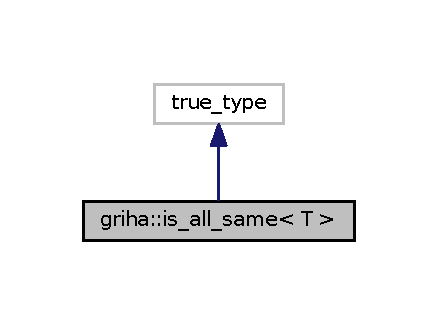
\includegraphics[width=210pt]{structgriha_1_1is__all__same_3_01_t_01_4__inherit__graph}
\end{center}
\end{figure}


Collaboration diagram for griha\+:\+:is\+\_\+all\+\_\+same$<$ T $>$\+:
\nopagebreak
\begin{figure}[H]
\begin{center}
\leavevmode
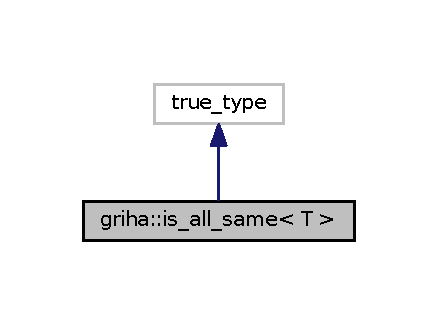
\includegraphics[width=210pt]{structgriha_1_1is__all__same_3_01_t_01_4__coll__graph}
\end{center}
\end{figure}


The documentation for this struct was generated from the following file\+:\begin{DoxyCompactItemize}
\item 
src/\hyperlink{type__traits_8h}{type\+\_\+traits.\+h}\end{DoxyCompactItemize}

\hypertarget{structgriha_1_1is__all__same_3_01_t_00_01_t_01_4}{}\section{griha\+:\+:is\+\_\+all\+\_\+same$<$ T, T $>$ Struct Template Reference}
\label{structgriha_1_1is__all__same_3_01_t_00_01_t_01_4}\index{griha\+::is\+\_\+all\+\_\+same$<$ T, T $>$@{griha\+::is\+\_\+all\+\_\+same$<$ T, T $>$}}


{\ttfamily \#include $<$type\+\_\+traits.\+h$>$}



Inheritance diagram for griha\+:\+:is\+\_\+all\+\_\+same$<$ T, T $>$\+:
% FIG 0


Collaboration diagram for griha\+:\+:is\+\_\+all\+\_\+same$<$ T, T $>$\+:
% FIG 1


The documentation for this struct was generated from the following file\+:\begin{DoxyCompactItemize}
\item 
src/\hyperlink{type__traits_8h}{type\+\_\+traits.\+h}\end{DoxyCompactItemize}

\hypertarget{structgriha_1_1is__all__same_3_01_t_00_01_t_00_01_args_8_8_8_01_4}{}\section{griha\+:\+:is\+\_\+all\+\_\+same$<$ T, T, Args... $>$ Struct Template Reference}
\label{structgriha_1_1is__all__same_3_01_t_00_01_t_00_01_args_8_8_8_01_4}\index{griha\+::is\+\_\+all\+\_\+same$<$ T, T, Args... $>$@{griha\+::is\+\_\+all\+\_\+same$<$ T, T, Args... $>$}}


{\ttfamily \#include $<$type\+\_\+traits.\+h$>$}



Inheritance diagram for griha\+:\+:is\+\_\+all\+\_\+same$<$ T, T, Args... $>$\+:
% FIG 0


Collaboration diagram for griha\+:\+:is\+\_\+all\+\_\+same$<$ T, T, Args... $>$\+:
% FIG 1


The documentation for this struct was generated from the following file\+:\begin{DoxyCompactItemize}
\item 
src/\hyperlink{type__traits_8h}{type\+\_\+traits.\+h}\end{DoxyCompactItemize}

\hypertarget{structgriha_1_1is__all__same_3_01_t_00_01_u_00_01_args_8_8_8_01_4}{}\section{griha\+:\+:is\+\_\+all\+\_\+same$<$ T, U, Args... $>$ Struct Template Reference}
\label{structgriha_1_1is__all__same_3_01_t_00_01_u_00_01_args_8_8_8_01_4}\index{griha\+::is\+\_\+all\+\_\+same$<$ T, U, Args... $>$@{griha\+::is\+\_\+all\+\_\+same$<$ T, U, Args... $>$}}


{\ttfamily \#include $<$type\+\_\+traits.\+h$>$}



Inheritance diagram for griha\+:\+:is\+\_\+all\+\_\+same$<$ T, U, Args... $>$\+:
% FIG 0


Collaboration diagram for griha\+:\+:is\+\_\+all\+\_\+same$<$ T, U, Args... $>$\+:
% FIG 1


The documentation for this struct was generated from the following file\+:\begin{DoxyCompactItemize}
\item 
src/\hyperlink{type__traits_8h}{type\+\_\+traits.\+h}\end{DoxyCompactItemize}

\hypertarget{structgriha_1_1is__one__of}{}\section{griha\+:\+:is\+\_\+one\+\_\+of$<$ T, Args $>$ Struct Template Reference}
\label{structgriha_1_1is__one__of}\index{griha\+::is\+\_\+one\+\_\+of$<$ T, Args $>$@{griha\+::is\+\_\+one\+\_\+of$<$ T, Args $>$}}


{\ttfamily \#include $<$type\+\_\+traits.\+h$>$}



The documentation for this struct was generated from the following file\+:\begin{DoxyCompactItemize}
\item 
src/\hyperlink{type__traits_8h}{type\+\_\+traits.\+h}\end{DoxyCompactItemize}

\hypertarget{structgriha_1_1is__one__of_3_01_t_01_4}{}\section{griha\+:\+:is\+\_\+one\+\_\+of$<$ T $>$ Struct Template Reference}
\label{structgriha_1_1is__one__of_3_01_t_01_4}\index{griha\+::is\+\_\+one\+\_\+of$<$ T $>$@{griha\+::is\+\_\+one\+\_\+of$<$ T $>$}}


{\ttfamily \#include $<$type\+\_\+traits.\+h$>$}



Inheritance diagram for griha\+:\+:is\+\_\+one\+\_\+of$<$ T $>$\+:
% FIG 0


Collaboration diagram for griha\+:\+:is\+\_\+one\+\_\+of$<$ T $>$\+:
% FIG 1


The documentation for this struct was generated from the following file\+:\begin{DoxyCompactItemize}
\item 
src/\hyperlink{type__traits_8h}{type\+\_\+traits.\+h}\end{DoxyCompactItemize}

\hypertarget{structgriha_1_1is__one__of_3_01_t_00_01_t_00_01_args_8_8_8_01_4}{}\section{griha\+:\+:is\+\_\+one\+\_\+of$<$ T, T, Args... $>$ Struct Template Reference}
\label{structgriha_1_1is__one__of_3_01_t_00_01_t_00_01_args_8_8_8_01_4}\index{griha\+::is\+\_\+one\+\_\+of$<$ T, T, Args... $>$@{griha\+::is\+\_\+one\+\_\+of$<$ T, T, Args... $>$}}


{\ttfamily \#include $<$type\+\_\+traits.\+h$>$}



Inheritance diagram for griha\+:\+:is\+\_\+one\+\_\+of$<$ T, T, Args... $>$\+:
% FIG 0


Collaboration diagram for griha\+:\+:is\+\_\+one\+\_\+of$<$ T, T, Args... $>$\+:
% FIG 1


The documentation for this struct was generated from the following file\+:\begin{DoxyCompactItemize}
\item 
src/\hyperlink{type__traits_8h}{type\+\_\+traits.\+h}\end{DoxyCompactItemize}

\hypertarget{structgriha_1_1is__one__of_3_01_t_00_01_u_00_01_args_8_8_8_01_4}{}\section{griha\+:\+:is\+\_\+one\+\_\+of$<$ T, U, Args... $>$ Struct Template Reference}
\label{structgriha_1_1is__one__of_3_01_t_00_01_u_00_01_args_8_8_8_01_4}\index{griha\+::is\+\_\+one\+\_\+of$<$ T, U, Args... $>$@{griha\+::is\+\_\+one\+\_\+of$<$ T, U, Args... $>$}}


{\ttfamily \#include $<$type\+\_\+traits.\+h$>$}



Inheritance diagram for griha\+:\+:is\+\_\+one\+\_\+of$<$ T, U, Args... $>$\+:
% FIG 0


Collaboration diagram for griha\+:\+:is\+\_\+one\+\_\+of$<$ T, U, Args... $>$\+:
% FIG 1


The documentation for this struct was generated from the following file\+:\begin{DoxyCompactItemize}
\item 
src/\hyperlink{type__traits_8h}{type\+\_\+traits.\+h}\end{DoxyCompactItemize}

\chapter{File Documentation}
\hypertarget{main_8cpp}{}\section{src/main.cpp File Reference}
\label{main_8cpp}\index{src/main.\+cpp@{src/main.\+cpp}}
{\ttfamily \#include $<$iostream$>$}\\*
{\ttfamily \#include $<$vector$>$}\\*
{\ttfamily \#include $<$list$>$}\\*
{\ttfamily \#include $<$tuple$>$}\\*
{\ttfamily \#include \char`\"{}print\+\_\+ip.\+h\char`\"{}}\\*
Include dependency graph for main.\+cpp\+:

\hypertarget{print__ip_8h}{}\section{src/print\+\_\+ip.h File Reference}
\label{print__ip_8h}\index{src/print\+\_\+ip.\+h@{src/print\+\_\+ip.\+h}}


File contains print\+\_\+ip function family.  


{\ttfamily \#include $<$iostream$>$}\\*
{\ttfamily \#include $<$type\+\_\+traits$>$}\\*
{\ttfamily \#include \char`\"{}type\+\_\+traits.\+h\char`\"{}}\\*
Include dependency graph for print\+\_\+ip.\+h\+:
% FIG 0
This graph shows which files directly or indirectly include this file\+:
% FIG 1
\subsection*{Namespaces}
\begin{DoxyCompactItemize}
\item 
 \hyperlink{namespacegriha}{griha}
\item 
 \hyperlink{namespacegriha_1_1details}{griha\+::details}
\end{DoxyCompactItemize}
\subsection*{Functions}
\begin{DoxyCompactItemize}
\item 
{\footnotesize template$<$typename Fwd\+It , typename CharT $>$ }\\std\+::basic\+\_\+ostream$<$ CharT $>$ \& \hyperlink{namespacegriha_1_1details_a0bb6a1ac333160e0c516e3c6af2ea8f6}{griha\+::details\+::print\+\_\+ip} (std\+::basic\+\_\+ostream$<$ CharT $>$ \&os, Fwd\+It f, Fwd\+It l)
\item 
{\footnotesize template$<$size\+\_\+t I, typename CharT , typename... Args$>$ }\\std\+::basic\+\_\+ostream$<$ CharT $>$ \& \hyperlink{namespacegriha_1_1details_aa298e5a3200d5b4b8f1833ba2736dabc}{griha\+::details\+::print\+\_\+ip} (std\+::basic\+\_\+ostream$<$ CharT $>$ \&os, const std\+::tuple$<$ Args... $>$ \&ip)
\item 
{\footnotesize template$<$typename CharT , typename... Args$>$ }\\std\+::basic\+\_\+ostream$<$ CharT $>$ \& \hyperlink{namespacegriha_1_1details_ae436fa4f3b9609914597737b2a61abc9}{griha\+::details\+::print\+\_\+ip} (std\+::basic\+\_\+ostream$<$ CharT $>$ \&os, const std\+::tuple$<$ Args... $>$ \&ip)
\item 
{\footnotesize template$<$typename CharT $>$ }\\std\+::basic\+\_\+ostream$<$ CharT $>$ \& \hyperlink{namespacegriha_a96b354d613153a0e77c127911a2e1ae0}{griha\+::print\+\_\+ip} (std\+::basic\+\_\+ostream$<$ CharT $>$ \&os, const std\+::basic\+\_\+string$<$ CharT $>$ \&ip)
\item 
{\footnotesize template$<$typename CharT , typename Char\+T2 , size\+\_\+t N$>$ }\\std\+::enable\+\_\+if\+\_\+t$<$ is\+\_\+character\+\_\+v$<$ Char\+T2 $>$, std\+::basic\+\_\+ostream$<$ CharT $>$ \& $>$ \hyperlink{namespacegriha_adb22fea7479742dc1c0a3d7c7995fc0b}{griha\+::print\+\_\+ip} (std\+::basic\+\_\+ostream$<$ CharT $>$ \&os, Char\+T2(\&ip)\mbox{[}N\mbox{]})
\item 
{\footnotesize template$<$typename CharT , typename IntT $>$ }\\std\+::enable\+\_\+if\+\_\+t$<$ std\+::is\+\_\+integral\+\_\+v$<$ IntT $>$, std\+::basic\+\_\+ostream$<$ CharT $>$ \& $>$ \hyperlink{namespacegriha_a4b0d906169c2b4c51fe323184bbc8f44}{griha\+::print\+\_\+ip} (std\+::basic\+\_\+ostream$<$ CharT $>$ \&os, IntT ip)
\item 
{\footnotesize template$<$typename CharT , typename IntT , size\+\_\+t N$>$ }\\std\+::enable\+\_\+if\+\_\+t$<$ std\+::is\+\_\+integral\+\_\+v$<$ IntT $>$ \&\&!is\+\_\+character\+\_\+v$<$ IntT $>$, std\+::basic\+\_\+ostream$<$ CharT $>$ \& $>$ \hyperlink{namespacegriha_aaa000663a06d833560a824a34a5ae42c}{griha\+::print\+\_\+ip} (std\+::basic\+\_\+ostream$<$ CharT $>$ \&os, IntT(\&ip)\mbox{[}N\mbox{]})
\item 
{\footnotesize template$<$typename CharT , typename ContT $>$ }\\std\+::enable\+\_\+if\+\_\+t$<$ std\+::is\+\_\+member\+\_\+function\+\_\+pointer\+\_\+v$<$ decltype(\&Cont\+T\+::cbegin)$>$ \&\&std\+::is\+\_\+member\+\_\+function\+\_\+pointer\+\_\+v$<$ decltype(\&Cont\+T\+::cend)$>$, std\+::basic\+\_\+ostream$<$ CharT $>$ \& $>$ \hyperlink{namespacegriha_a11ead801358ba902938ff6dcb9ac4da2}{griha\+::print\+\_\+ip} (std\+::basic\+\_\+ostream$<$ CharT $>$ \&os, const ContT \&ip)
\item 
{\footnotesize template$<$typename CharT , typename... Args$>$ }\\std\+::enable\+\_\+if\+\_\+t$<$ is\+\_\+all\+\_\+same\+\_\+v$<$ Args... $>$, std\+::basic\+\_\+ostream$<$ CharT $>$ \& $>$ \hyperlink{namespacegriha_acd1e1da8a6524b3c7521bc759da1c3ae}{griha\+::print\+\_\+ip} (std\+::basic\+\_\+ostream$<$ CharT $>$ \&os, const std\+::tuple$<$ Args... $>$ \&ip)
\end{DoxyCompactItemize}


\subsection{Detailed Description}
File contains print\+\_\+ip function family. 

This function can print IP address represented by std\+::string object, string literal as {\ttfamily \char`\"{}192.\+168.\+1.\+1\char`\"{}} with null-\/terminated symbol, integral type as {\ttfamily char}, {\ttfamily short}, {\ttfamily int}, {\ttfamily long} and etc, array of values of integral type, and container and tuple of same types elements

\begin{DoxyAuthor}{Author}
griha \href{mailto:gpgolikov@gmail.com}{\tt gpgolikov@gmail.\+com} 
\end{DoxyAuthor}

\hypertarget{type__traits_8h}{}\section{src/type\+\_\+traits.h File Reference}
\label{type__traits_8h}\index{src/type\+\_\+traits.\+h@{src/type\+\_\+traits.\+h}}
{\ttfamily \#include $<$type\+\_\+traits$>$}\\*
Include dependency graph for type\+\_\+traits.\+h\+:
\nopagebreak
\begin{figure}[H]
\begin{center}
\leavevmode
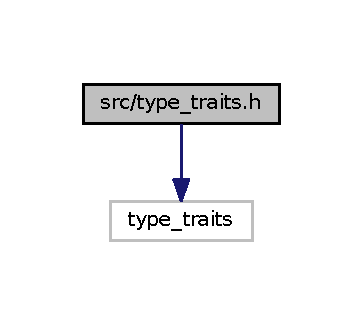
\includegraphics[width=174pt]{type__traits_8h__incl}
\end{center}
\end{figure}
This graph shows which files directly or indirectly include this file\+:
\nopagebreak
\begin{figure}[H]
\begin{center}
\leavevmode
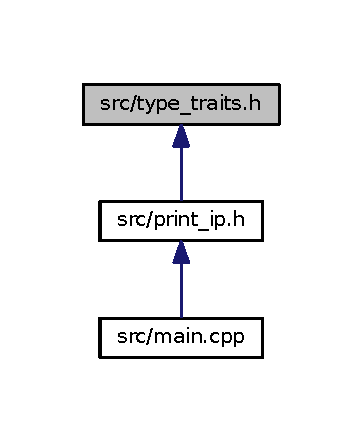
\includegraphics[width=174pt]{type__traits_8h__dep__incl}
\end{center}
\end{figure}
\subsection*{Classes}
\begin{DoxyCompactItemize}
\item 
struct \hyperlink{structgriha_1_1is__one__of}{griha\+::is\+\_\+one\+\_\+of$<$ T, Args $>$}
\item 
struct \hyperlink{structgriha_1_1is__one__of_3_01_t_01_4}{griha\+::is\+\_\+one\+\_\+of$<$ T $>$}
\item 
struct \hyperlink{structgriha_1_1is__one__of_3_01_t_00_01_t_00_01_args_8_8_8_01_4}{griha\+::is\+\_\+one\+\_\+of$<$ T, T, Args... $>$}
\item 
struct \hyperlink{structgriha_1_1is__one__of_3_01_t_00_01_u_00_01_args_8_8_8_01_4}{griha\+::is\+\_\+one\+\_\+of$<$ T, U, Args... $>$}
\item 
struct \hyperlink{structgriha_1_1is__all__same}{griha\+::is\+\_\+all\+\_\+same$<$ Args $>$}
\item 
struct \hyperlink{structgriha_1_1is__all__same_3_01_t_01_4}{griha\+::is\+\_\+all\+\_\+same$<$ T $>$}
\item 
struct \hyperlink{structgriha_1_1is__all__same_3_01_t_00_01_t_01_4}{griha\+::is\+\_\+all\+\_\+same$<$ T, T $>$}
\item 
struct \hyperlink{structgriha_1_1is__all__same_3_01_t_00_01_u_00_01_args_8_8_8_01_4}{griha\+::is\+\_\+all\+\_\+same$<$ T, U, Args... $>$}
\item 
struct \hyperlink{structgriha_1_1is__all__same_3_01_t_00_01_t_00_01_args_8_8_8_01_4}{griha\+::is\+\_\+all\+\_\+same$<$ T, T, Args... $>$}
\end{DoxyCompactItemize}
\subsection*{Namespaces}
\begin{DoxyCompactItemize}
\item 
 \hyperlink{namespacegriha}{griha}
\end{DoxyCompactItemize}
\subsection*{Variables}
\begin{DoxyCompactItemize}
\item 
{\footnotesize template$<$typename T , typename... Args$>$ }\\constexpr auto \hyperlink{namespacegriha_a4143946f18648e253a58b1ecd283a657}{griha\+::is\+\_\+one\+\_\+of\+\_\+v} = is\+\_\+one\+\_\+of$<$T, Args...$>$\+::value
\item 
{\footnotesize template$<$typename... Args$>$ }\\constexpr auto \hyperlink{namespacegriha_a3c9eb374b11b670884dfabc46b7bbc23}{griha\+::is\+\_\+all\+\_\+same\+\_\+v} = is\+\_\+all\+\_\+same$<$Args...$>$\+::value
\item 
{\footnotesize template$<$typename T $>$ }\\constexpr auto \hyperlink{namespacegriha_af6e5a84a5dad7d2123491eb7124aa2e3}{griha\+::is\+\_\+character\+\_\+v} = is\+\_\+one\+\_\+of\+\_\+v$<$std\+::decay\+\_\+t$<$T$>$, char, wchar\+\_\+t, char16\+\_\+t, char32\+\_\+t$>$
\end{DoxyCompactItemize}

%--- End generated contents ---

% Index
\backmatter
\newpage
\phantomsection
\clearemptydoublepage
\addcontentsline{toc}{chapter}{Index}
\printindex

\end{document}
